\chapter{Data Samples and Event Selection}\label{ch:data}
The data used in this analysis were collected in late 2017 by the CMS Experiment during Run II of the LHC. At this time, the LHC delivered two sets of \pp collisions, at \serag (2017G) and at \serah (2017H). This chapter details the information related to data collection and Monte Carlo simulations associated with these data taking periods. Details regarding the object identification criteria and event selection are also provided.

%%%%%%%%%%%%%%%%%%%%%%%%%%%%%%%%%%%%%%
%%%     Dataset 
%%%%%%%%%%%%%%%%%%%%%%%%%%%%%%%%%%%%%%


\section{Datasets}\label{ch:data:dataset}
Data used in this analysis are from the LHC run eras 2017G and 2017H, consisting of \pp collisions at \serag with integrated luminosity $\mathcal{L}=\lumig$ and \serah with integrated luminosity $\mathcal{L}=\lumih$, respectively. Names of the data streams and relevant run era and reconstruction version identifications are listed in Table~\ref{tab:dataset13} and Table~\ref{tab:dataset5}. 
%%%% 5 TeV datastreams
\begin{table}[htbp]
\begin{center}
\scalebox{1.0}{
\begin{tabular}{l l}
\hline {Data stream} &  {Run \& version}  \\
\hline \hline
SingleMuon      &       Run2017G-17Nov2017-v1   \\
HighEGJet       &       Run2017G-17Nov2017-v2          \\
\hline
\end{tabular}}
\end{center}

\caption{Data streams and the respective run and reconstruction versions for the 2017G (5.02 \TeV) data taking.}
\label{tab:dataset5}
\end{table}

%%%% 13 TeV datastreams
\begin{table}[htbp]
\begin{center}
\scalebox{1.0}{
\begin{tabular}{l l}
\hline {Data stream} &  {Run \& version}  \\
\hline \hline
SingleMuon      &       Run2017H-17Nov2017-v2   \\
HighEGJet       &       Run2017H-17Nov2017-v1          \\
\hline

\end{tabular}}
\end{center}

\caption{Data streams and the respective run and reconstruction versions for the 2017H (13 \TeV) data taking.}
\label{tab:dataset13}
\end{table}



\section{Triggers}\label{ch:data:triggers}
All events considered must have at least one lepton selected by the relevant trigger path. For muons, the kinematic requirement is $\pt>17\GeV$ and $|\eta|<2.4$ for both \serag and \serah. For electrons, the kinematic requirement is $\pt>20\GeV$ ($\pt>17\GeV$) and $|\eta|<2.5$ for \serag (\serah). Additional isolation and reconstruction quality criteria, which are less restrictive than the offline selection criteria, are applied at the trigger level. Names of the trigger paths are listed in  Table~\ref{tab:triggers}

%%%% triggers
\begin{table}[htbp]
\begin{center}
\begin{tabular}{c c}
\hline
\serah    & \serag  \\
\hline \hline
\verb|HLT_HIEle20_WPLoose_Gsf|  & \verb|HLT_HIEle17_WPLoose_Gsf| \\
\hline
\verb|HLT_HIMu17|   &  \verb|HLT_HIMu17| \\
\hline
\end{tabular}
\end{center}
\caption{Data streams and reconstruction versions for the 2017G (5.02 \TeV) data taking.}
\label{tab:triggers}
\end{table}

%%%%%%%%%%%%%%%%%%%%%%%%%%%%%%%%%%%%%%
%%%     Lumi Calibration 
%%%%%%%%%%%%%%%%%%%%%%%%%%%%%%%%%%%%%%

\section{Luminosity}\label{ch:lumi}
Data used for physics analyses are required to pass the quality certification regarding operation of detector subsystems during the data taking period. 
% The list of data taking periods with highest quality requirements are compiled into a good run list .
% The JSON files containing the selected data segments for 2017G (\serag) and 2017H (\serah) are: \\
% \centerline{\texttt{\small Cert\_306546-306826\_5TeV\_EOY2017ReReco\_Collisions17\_JSON.txt}}
% \centerline{\texttt{\small Cert\_306896-307082\_13TeV\_PromptReco\_Collisions17\_JSON\_LowPU\_lowPU.txt}}
%
The 2017G and 2017H data taking periods are notable for the LHC conditions producing very few additional collisions in the concurrent or adjacent bunch crossings. These additional collisions are referred to as pileup events. Pileup conditions during the data taking periods are shown in Figure~\ref{fig:data:lumiPU13}, with an average of $\langle\mu\rangle=3$ collisions per bunch crossing. The instantaneous luminosity per day is shown in Figure~\ref{fig:data:lumiperday5}. Uncertainties on the luminosity measurement are 1.7\% (3.5\%) for the certified data at \serah (\serag). The total integrated luminosity collected by the data streams during \serag and \serah are listed in Table~\ref{tab:lumis}~\cite{LumiPOGNumbers}.
\begin{figure}[htbp]
\centering
  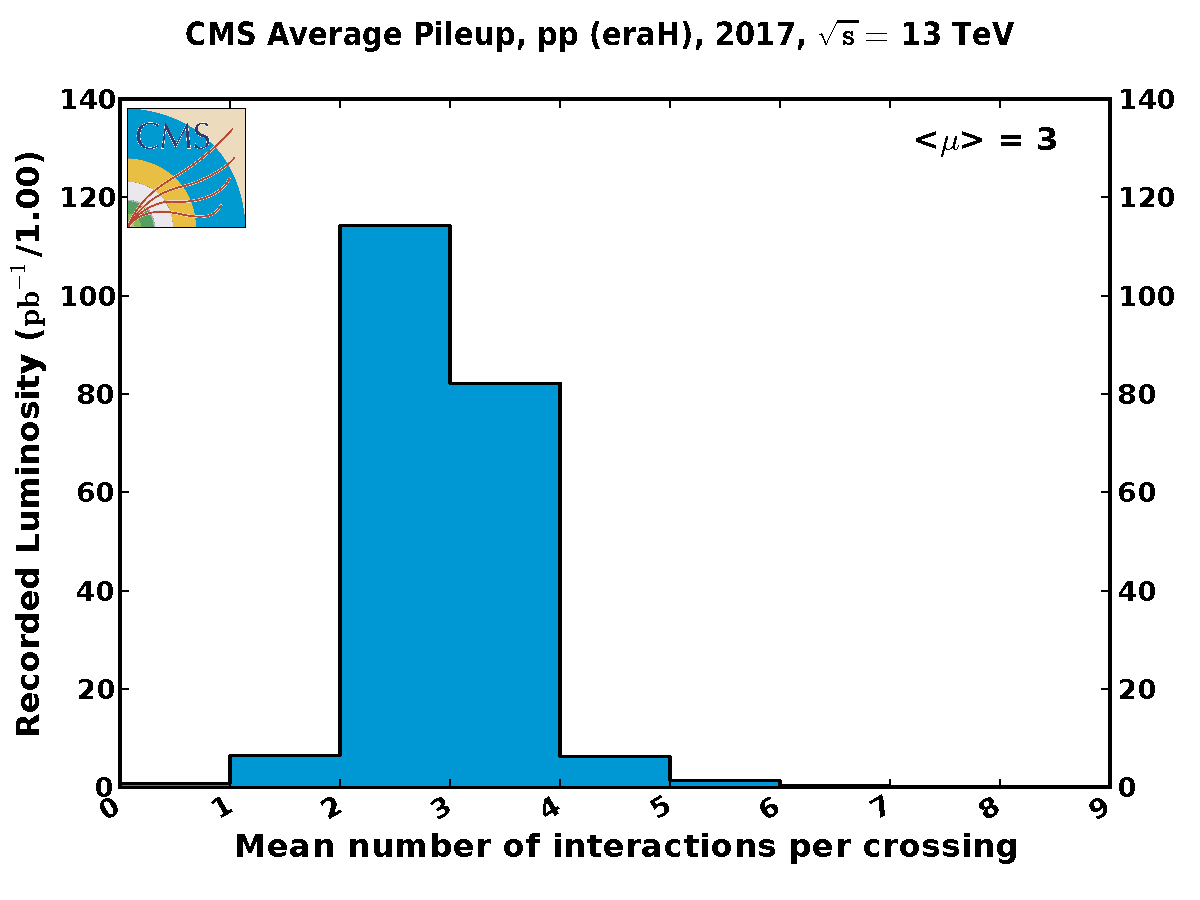
\includegraphics[width=0.75\textwidth]{plots/Data/pileup_pp_lowPU_2017.pdf}
  %https://cds.cern.ch/record/40524
  \caption{Distribution of the number of interactions per bunch crossing for the low pileup \sh (2017H) data taking period. The average number of interactions per crossing is $<\mu> = 3$~\cite{LumiCalibTwiki}.}
  \label{fig:data:lumiPU13}
\end{figure}

\begin{figure}[htbp]
\centering
  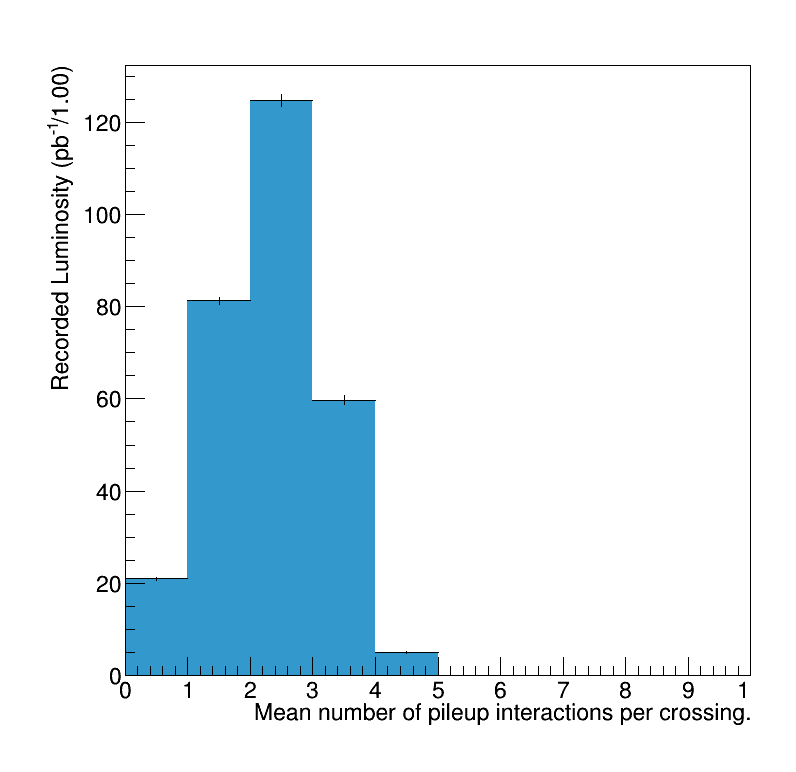
\includegraphics[width=0.75\textwidth]{plots/Data/pileup_5TeV.png}
  %https://cds.cern.ch/record/40524
  \caption{Distribution of the number of interactions per bunch crossing for the \sg (2017G) data taking period. The average number of interactions per crossing is $<\mu> = 2$~\cite{LumiCalibTwiki}.}
  \label{fig:data:lumiPU5}
\end{figure}
\begin{figure}[htbp]
\centering
  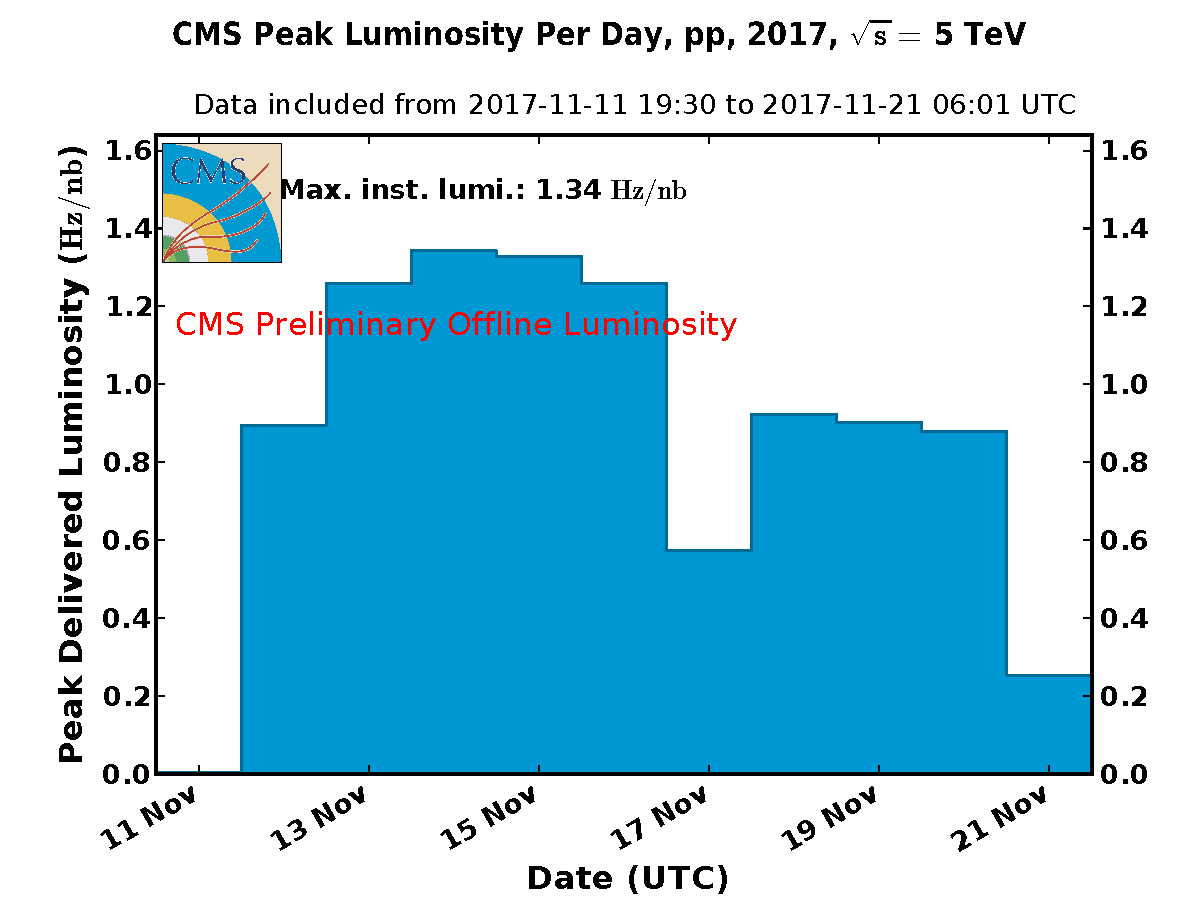
\includegraphics[width=0.6\textwidth]{plots/Data/peak_lumi_per_day_pp_2017_5TeV_NormtagLumi.pdf}
  %https://cds.cern.ch/record/40524
  \caption{Peak instantaneous luminosity per day during the \sg (2017G) data taking period~\cite{LumiCalibTwiki}.}
  \label{fig:data:lumiperday5}
\end{figure}
%%%% lumi values
\begin{table}[htbp]
\begin{center}
\scalebox{1.0}{
\begin{tabular}{c c c}
\hline {\s [\TeV]} & {Run Era} &  {Luminosity [\invpb]}  \\
\hline \hline
5.02  & 2017G    &   $199.2 \pm   3.39$   \\
13    & 2017H    &   $291.1 \pm  11.64$   \\
\hline
\end{tabular}}
\end{center}

\caption{Datasets and their respective integrated luminosity measurements.}
\label{tab:lumis}
\end{table}

%% Is there a specific thing to cite if you use brilcalc to get the lumi out of the trigger path


%%%%%%%%%%%%%%%%%%%%%%%%%%%%%%%%%%%%%%
%%%     Simulated Samples & info 
%%%%%%%%%%%%%%%%%%%%%%%%%%%%%%%%%%%%%%

\section{Simulated samples}\label{ch:data:sim}
Several simulated Monte Carlo (MC) samples are used in the descriptions of signal and background processes. The \Wpm and \Z boson signal events are simulated at next-to-leading order (NLO) with up to two outgoing partons at Born level by \MGvATNLO~2.3.3~\cite{Alwall:2014hca}. An additional set of simulations of the \Wpm and \Z boson signal processes are provided at NLO by \POWHEG~2.0~\cite{Alioli:2008gx,Frixione:2007vw,powheg:2010,Alioli:2010xd} for the \Wpm and \MINLO~\cite{Hamilton:2012rf} for the \Z boson. Background samples (di-boson and \ttbar) are also simulated with \POWHEG~2.0. Underlying event modeling, parton showering, hadronization, and final state radiation are done by \PYTHIA~8.230~\cite{Sjostrand:2014zea}, using tune CP5~\cite{Sirunyan:2019dfx} and default parton distribution functions (PDFs) provided by NNPDF3.1~\cite{Ball:2017nwa}. Primary sample names and their respective production cross sections are listed in Table~\ref{tab:allSamples5} (Table~\ref{tab:allSamples13}) for \serag (\serah).

The distribution of pileup interactions is simulated to match the corresponding conditions in data. For all simulated samples, simulation of detector response is performed by \GEANTfour~\cite{Agostinelli:2002hh}, with full event reconstruction being done using the same algorithms used to reconstruct data. Object and event reconstruction was described in Chapter~\ref{ch:reco}. 

%%% 5 TeV MCs
\begin{table}[htbp]
\begin{center}
\scalebox{0.9}{
\begin{tabular}{llr}
\hline
{Sample name} & {Generator} &{~~~Cross section~[pb]} \\
\hline \hline
W+Jets & \aMCATNLO & 21159 \\
\hline
$WW\to 2\ell 2\nu$  & \POWHEG & 2.52 \\
$WZ\to 3\ell \nu$  & \POWHEG & 1.23 \\
$ZZ\to 4\ell$  & \POWHEG & 2.75 \\
$ZZ\to 2\ell 2\nu$  & \POWHEG & 2.75 \\
\hline
\ttbar  & \POWHEG &  69.5 \\
\hline
DY+jets$\to\ell\ell$ ~~~ & \aMCATNLO & 2141  \\
\hline
\end{tabular}}
\end{center}
\caption{Names and cross sections of simulated samples corresponding to run era 2017G (\serag).}
\label{tab:allSamples5}
\end{table}


%%% 13 TeV MCs
\begin{table}[htbp]
\begin{center}
\scalebox{0.9}{
\begin{tabular}{llr}
\hline
{Sample name}  & {Generator}& {~~~Cross section~[pb]} \\
\hline \hline
$W$+0 jets & \aMCATNLO & 49397\\
$W$+1 jets  &\aMCATNLO & 8087 \\
$W$+2 jets  & \aMCATNLO & 3176 \\
\hline
ZZ  & \POWHEG  & 16.523 \\
$WZ\to 3\ell\nu$  & \POWHEG  & 4.912 \\
$WZ\to 2\ell 2\nu$  & \POWHEG  & 12.6 \\
\hline
$\ttbar \to 2\ell 2\nu$  & \POWHEG  & 88.29 \\
$\ttbar \to \mathrm{semileptonic}$ ~~~ & \POWHEG  & 365.35 \\
$\ttbar \to \mathrm{hadronic}$  & \POWHEG  & 377.96 \\
\hline
DY+jets$\to\ell\ell$  & \aMCATNLO & 6225.42 \\
\hline
\end{tabular}}
\end{center}
\caption{Names and cross sections of simulated samples corresponding to run era 2017H (\serah).}
\label{tab:allSamples13}
\end{table}



% %%% 5 TeV MCs
% \begin{table}[htbp]
% \begin{center}
% \scalebox{0.9}{
% \begin{tabular}{lrr}
% \hline
% {Sample name} & {Cross section~[pb]} \\
% \hline \hline
% WJetsToLNu\_TuneCP5\_5020GeV-amcatnloFXFX-pythia8 & 21159 \\
% \hline
% WWTo2L2Nu\_NNPDF31\_TuneCP5\_5p02TeV-powheg-pythia8 & 2.52 \\
% WZTo3LNU\_NNPDF30\_TuneCP5\_5p20TeV-powheg & 1.23 \\
% ZZTo4L\_5p02TeV\_powheg\_pythia8 & 2.75 \\
% ZZTo2L2Nu\_5p02TeV\_powheg\_pythia8 & 2.75 \\
% \hline
% TT\_TuneCP5\_5p02TeV-powheg-pythia8 &  69.5 \\
% \hline
% DYJetsToLL\_MLL-50\_TuneCP5\_5020GeV-amcatnloFXFX-pythia8 & 2141  \\
% \hline
% \end{tabular}}
% \end{center}
% \caption{Names and cross sections of simulated samples corresponding to run era 2017G (5.02 TeV).}
% \label{tab:allSamples5}
% \end{table}


% %%% 13 TeV MCs
% \begin{table}[htbp]
% \begin{center}
% \scalebox{0.9}{
% \begin{tabular}{lrr}
% \hline
% {Sample name} & {Cross section~[pb]} \\
% \hline \hline
% WJetsToLNu\_0J\_TuneCP5\_13TeV-amcatnloFXFX-pythia8 & 49397\\
% WJetsToLNu\_1J\_TuneCP5\_13TeV-amcatnloFXFX-pythia8 & 8087 \\
% WJetsToLNu\_2J\_TuneCP5\_13TeV-amcatnloFXFX-pythia8 & 3176 \\
% \hline
% ZZ\_TuneCP5\_13TeV-pythia8  & 16.523 \\
% WZTo3LNu\_TuneCP5\_13TeV-powheg-pythia8  & 4.912 \\
% WWTo2L2Nu\_TuneCP5\_13TeV-powheg-pythia8  & 12.6 \\
% \hline
% TTTo2L2Nu\_TuneCP5\_13TeV-powheg-pythia8  & 88.29 \\
% TTToSemiLeptonic\_TuneCP5\_13TeV-powheg-pythia8  & 365.35 \\
% TTToHadronic\_TuneCP5\_13TeV-powheg-pythia8  & 377.96 \\
% \hline
% DYJetsToLL\_M-50\_TuneCP5\_13TeV-amcatnloFXFX-pythia8 & 6225.42 \\
% \hline
% \end{tabular}}
% \end{center}
% \caption{Names and cross sections of simulated samples corresponding to run era 2017H (13 TeV).}
% \label{tab:allSamples13}
% \end{table}




%%%%%%%%%%%%%%%%%%%%%%%%%%%%%%%%%%%%%%
%%%     Event Selection
%%%%%%%%%%%%%%%%%%%%%%%%%%%%%%%%%%%%%%
\section{Event Selection \& Fiducial Region}
 \subsubsection{Reconstructed}
Preliminary \Wpm and \Z boson event candidates are identified by the presence of at least one lepton identified by the single electron and single muon triggers described in Section~\ref{ch:data:triggers}. These are further selected by applying the offline electron or muon reconstruction identification criteria described in Section~\ref{ch:IdIso}. 
A \Z boson event requires the presence a pair of oppositely charged leptons ($e^{+}e^{-}$ or $\mu^{+}\mu^{-}$), at least one of the leptons being identified by the trigger, and each of the leptons fulfilling the ID requirements in Section~\ref{ch:IdIso}, and an invariant mass of \masswindow. 
Selection of a \Wp or \Wm boson candidate requires one charged lepton identified by the trigger and passing all ID requirements in Section~\ref{ch:IdIso}. A veto is applied to events containing additional leptons passing a loose identification requirement. 

% Additionally, \Wpm events are required to have an invariant mass $\mt > 40\GeV$, with \mt defined by: 
% $\mt = \sqrt{ 2 \pt \met ( 1 - \cos(\Delta\phi) ) }$, where $\Delta\phi$ is the angle between the lepton and \vmet in the transverse plane.

\subsubsection{Fiducial Region}
The fiducial region for the \Wpm and \Z boson acceptance at generator-level emulates the selection at reconstruction level. This requires kinematic cuts $\pt > 25 \GeV$ and $|\eta| < 2.4$ for all charged leptons. Additionally, the \Z boson fiducial region includes a requirement on the dilepton mass: \masswindow. The fiducial region for the \W boson includes the transverse mass requirement $\mt>40\GeV$.


%%%%%%%%%%%%%%%%%%%%%%%%%%%%%%%%%%%%%%
%%%     object definition
%%%%%%%%%%%%%%%%%%%%%%%%%%%%%%%%%%%%%%
\section{Object Identification}\label{ch:IdIso}
The \W and \Z boson candidates are identified by the presence of one or two, respectively, well-identified leptons passing a strong set of criteria ensuring proper reconstruction and identification. This section contains a description of the identification requirements for the \wlnu and \zll signal leptons, as well as the requirements for the lepton veto for the \Wpm boson selection.

\subsection{Isolation}\label{ch:id:iso}
One of the most important observables used to separate the leptons from \Wp and \Wm boson events from QCD background is the isolation. Isolated leptons have little other activity within a cone of $\Delta R < 0.3$, and leptons from \wlnu decays are generally isolated. The isolation of a lepton is constructed from the sum of all charged and neutral hadrons and ECAL deposits within $\Delta R < 0.3$ of the lepton, as shown in Equation~\ref{eq:pfiso}. 
\begin{equation}
    I_{PF} = \frac{1}{\pt}\sum_{\Delta R<0.3}( \pt^{h^0} + \pt^{h^\pm} +  \pt^{\gamma})
    \label{eq:pfiso}
\end{equation}
The individual contributions to the PF isolation are the sums of corresponding particle types which fall within a cone of $\Delta R < 0.4$.
% \begin{equation}
%     \Delta R = \sqrt{\Delta\eta^2+\Delta\phi^2}
%     \label{eq:dR}
% \end{equation}
% Neutral particle contributions due to pileup are estimated by computing charged hadron contributions from pileup vertices and scaling it by 0.5. The scaling factor was determined using simulation. This pileup contribution is subtracted from the total neutral particle energy sum to get the neutral particle isolation, which is limited to be $\geq0$.

\subsection{Electrons}\label{ch:IdIso:Ele}
Electrons originating from candidate \Wp, \Wm, and \Z bosons are required to pass the standard cut-based identification with medium working point. Backgrounds producing electron-like signatures include overlapping charged and neutral pions, pions showering in the ECAL, and jets, and the selection criteria are designed to exclude these. The thresholds for observables required to pass this requirement are listed in Table~\ref{tab:Data:Sel:Ele}~\cite{EgammaIDIsoCuts}. Descriptions of the observables are provided below. The \Wpm boson selection requires the absence of additional leptons in the event. The veto is performed with leptons fulfilling the loose working point identification requirements, with criteria for electrons listed in Table~\ref{tab:Data:Sel:EleVeto}. 
\subsubsection{Electron Observables}
\begin{itemize}
    \item \textbf{($\Delta\eta_{In}$,$\Delta\phi_{In}$):} Geometric matching of the ECAL supercluster and electron GSF track, extrapolated to the vertex. Real electrons are well-matched since they come from the same object. 
    \item \textbf{$\sigma_{i\eta i\eta}$:} Shape of the shower in the ECAL. Electrons can be discriminated from jets by the evolution of the shower in the 5x5 crystal region around the seed.
    \item \textbf{H/E:} Ratio of energy deposited in HCAL to ECAL. Electrons tend to deposit most of their energy in the ECAL, while jets deposit substantial amounts their of energy in the HCAL.
    \item \textbf{$|d_{0,bs}|$,~$|d_{z,bs}|$:} Impact parameters are defined as the distance of closest approach of the track to the vertex. Requiring an impact parameter cut removes electrons from displaced vertices.
    \item \textbf{$|1/E-1/p|$:} Electron energy measured in ECAL is compatible with momentum measured in tracker.
    \item \textbf{Number of Missing Hits}: Number of missing tracker hits in tracker layer
    \item \textbf{Isolation:} Requiring that electrons be isolated reduces the number of jets reconstructed as electrons.
    \item \textbf{Conversion probability}: Photons converting to electron-positron pairs are a source of isolated electrons. Electrons from photon conversion are identified by fitting $e^+e^-$ pairs to a common vertex.
\end{itemize}

%%%% Table containing the Ele ID+Iso cuts
\begin{table}[htbp]
\begin{center}
\scalebox{0.8}{
\begin{tabular}{|c|c|c|}
\hline
Observable & Barrel & Endcap \\
\hline \hline
$p_T$ & \multicolumn{2}{c|}{$> 25$ \GeV} \\ \hline % OK
$|\eta|$ & \multicolumn{2}{c|}{$< 2.4$}\\ \hline% OK
$\Delta\eta_{In}$ & $< 0.0032$ & $< 0.00632$\\ \hline% OK
$\Delta\phi_{In}$ & $< 0.0547$ & $< 0.0394$\\ \hline% OK
$\sigma_{i\eta i\eta}$ & $<  0.0106$ & $< 0.0387$\\ \hline% OK
H/E & $< 0.046+1.16/E_{SC}+0.0324\rho/E_{SC}$ & $< 0.0275+2.52/E_{SC}+0.183\rho/E_{SC}$\\ \hline%
$|d_{0,bs}|$ & $< 0.05$ & $< 0.10$\\ \hline% OK
$|d_{z,bs}|$ & $< 0.10$ & $< 0.20$\\ \hline% OK
$|1/E-1/p|$ & $< 0.184$& $< 0.0721$\\ \hline% OK
$\mathrm{Iso_{PF}}/$\pt &$< 0.0478+0.506/p_{\mathrm{T},ele}$ &$< 0.0658+0.963/p_{\mathrm{T},ele}$ \\ \hline
Missing Hits & \multicolumn{2}{c|}{$\leq 1$}\\ \hline
\multicolumn{3}{|c|}{Pass conversion veto}\\
\hline
\end{tabular} }
\end{center}
\caption{Reconstructed identification and isolation criteria fulfilling the medium cut-based ID for electron selection.}
\label{tab:Data:Sel:Ele}
\end{table}

%% Table containing the Electron ID+Iso Veto cuts
%% Cut Type
\begin{table}[htbp]
\begin{center}
\scalebox{0.8}{
\begin{tabular}{|c|c|c|} %%%% Table needs vertical lines
\hline
Observable & Barrel & Endcap \\
\hline \hline
$p_T$ & \multicolumn{2}{c|}{$> 25$ \GeV} \\ \hline % OK
$|\eta|$ & \multicolumn{2}{c|}{$< 2.4$}\\ \hline% OK
$\Delta\eta_{In}$ & $< 0.00463$ & $< 0.00814$\\ \hline
$\Delta\phi_{In}$ & $< 0.148$ & $< 0.19$\\ \hline
$\sigma_{i\eta i\eta}$ & $< 0.0126$ & $< 0.0457$\\ \hline
H/E & $< 0.05+1.16/E_{SC}+0.0324\rho/E_{SC}$ & $< 0.05+2.54/E_{SC}+0.183\rho/E_{SC}$\\ \hline%
$|d_{0,bs}|$ & $< 0.05$ & $< 0.10$\\ \hline
$|d_{z,bs}|$ & $< 0.10$ & $< 0.20$\\ \hline
$|1/E-1/p|$ & $<0.209$& $< 0.132$\\ \hline
$\mathrm{Iso_{PF}}/$\pt &$< 0.198+0.506/p_{T,ele}$ &$< 0.203+0.963/p_{T,ele}$ \\ \hline
Missing Hits & $\leq 2$ & $\leq 3$\\ \hline
\multicolumn{3}{|c|}{Pass conversion veto}\\
\hline
\end{tabular}}
\end{center}
\caption{Reconstructed identification and isolation criteria fulfilling the loose cut-based ID for electron selection used as a veto on \Wpm events with additional leptons present.}
\label{tab:Data:Sel:EleVeto}
\end{table}

\subsection{Muons}\label{ch:IdIso:Mu}
Muons originating from a candidate \Wpm or \Z boson are required to pass the standard cut-based identification with tight working point with tight working point requirement on the muon PF isolation. The thresholds for observables required to pass this requirement are listed in Table~\ref{tab:Data:Sel:Mu}~\cite{MuonIDIsoCuts}. Descriptions of the observables are provided below. As in the electron channel, the \Wpm boson selection requires the absence of additional leptons in an event which pass the loose cut-based ID. The criteria for muons is listed in Table~\ref{tab:Data:Sel:Mu:Veto}. 
%%%%%%%%%%%%%%%%%%%%%%%%%%%%%%%%%%%%%
\subsubsection{Muon Observables}
\begin{itemize}
    \item \textbf{Global Muon \& PF Muon:} Muon candidate is successfully reconstructed by these algorithms
    \item \textbf{$\chi^2/$ndof:} Quality of the muon track fit, require convergence of the fit.
    \item \textbf{Number of Valid Hits:} Number of muon system hits included in the global muon reconstruction. Global muons rarely have 0 valid hits.
    \item \textbf{Number of Matched Stations:} Number of muon segments in the muon stations
    \item \textbf{Number of Pixel Hits:} Activity in the pixel tracker associated with the muon removes muons from backgrounds such as cosmic rays and decay-in-flight of pions and kaons. 
    \item \textbf{Number of Tracker Hits:} Similar to the pixel tracker requirements, the total number of tracker hits can further reduce backgrounds from decay-in-flight.
    \item \textbf{$|d_{0,bs}|$,~$|d_{z,bs}|$:} Impact parameters $d_0$ and $d_z$ are defined as the distance of closest approach of a track to the primary interaction vertex. Removes muons from displaced vertices and cosmic rays. 
    \item \textbf{Isolation:} Muons originating from heavy flavor decays often have other leptons and light mesons nearby, and are therefore less isolated.
\end{itemize}

%%%% Table containing the Ele ID+Iso cuts
\begin{table}[htbp]
\begin{center}
\scalebox{0.8}{
\begin{tabular}{|c|c|}
\hline
Observable & Value/Range \\
\hline \hline
\pt & > 25 GeV \\ \hline % OK
$|\eta|$ & $< 2.4$\\ \hline% OK
ID & ~GlobalMuon~ \\ \hline% OK
ID & ~PFMuon~\\ \hline% OK
$\chi^2/$ndof & $< 10$\\ \hline% OK
~\# Valid Mu Hits ~ & $\geq 1$\\ \hline%
~\# Matched Stations ~& $\geq 2$\\ \hline%
~\# Tracker Layers ~& $\geq 6$\\ \hline%
~\# Valid Pixel Hits~ & $\geq 1$\\ \hline%
$|d_{0,bs}|$ & < 0.2 \\ \hline% OK
$|d_{z,bs}|$ & < 0.5 \\ \hline% OK
$\mathrm{Iso_{PF}}/$\pt &$< 0.15$\\
\hline
\end{tabular}}
\end{center}
\caption{Reconstructed identification and isolation criteria fulfilling the cut-based ID with tight isolation requirement for muon selection.}
\label{tab:Data:Sel:Mu}
\end{table}
%%%% Table containing the Ele ID+Iso cuts
\begin{table}[htbp]
\begin{center}
\scalebox{0.8}{
\begin{tabular}{|c|c|c|}
\hline
Observable & Value/Range \\
\hline \hline
\pt & > 10 GeV \\ \hline % OK
$|\eta|$ & < 2.4\\ \hline% OK
ID & \textsc{GlobalMuon} \textbf{OR} \textsc{TrackerMuon}\\ \hline% OK
ID & \textsc{PFMuon}\\ 
\hline
\end{tabular}}
\end{center}
\caption{Reconstructed identification and isolation criteria for identifying additional muons used as a veto on \Wpm boson events.}
\label{tab:Data:Sel:Mu:Veto}
\end{table}

